\documentclass[11pt]{article}
\usepackage[a4paper,margin=18mm]{geometry}
\usepackage{amsmath,amssymb}
\usepackage{booktabs,array}
\usepackage{enumitem}
\usepackage{tikz}
\usetikzlibrary{arrows.meta,positioning,fit}
\usepackage[hidelinks]{hyperref}
\setlength{\parindent}{0pt}
\setlength{\parskip}{5pt}
\setlist[enumerate]{leftmargin=1.8em,itemsep=2pt,topsep=3pt}
\newcommand{\q}[2]{\vspace{0.5em}\noindent\textbf{Question #1}\if\relax\detokenize{#2}\relax\else\ \textit{(#2)}\fi\par}
\newcommand{\opts}{\textbf{Options:}}
\newcommand{\contexthead}[1]{\vspace{0.6em}\noindent\textbf{Context for Questions #1}\par}

\begin{document}

\begin{center}
{\Large\bfseries Large Language Models -- Extracted Question Papers}\\[2mm]
{\small Administrative prompts, question IDs, marks, answer keys, section metadata, and other non-question data have been omitted.}
\end{center}

\section*{Paper 1}

\q{2}{MSQ}
Which statements are true about traditional attention used in sequence-to-sequence models?

\opts
\begin{enumerate}[label=(\alph*)]
\item The decoder decides which encoder states are important.
\item Attention weights are computed over all decoder hidden states.
\item The context vector is a weighted sum of encoder states.
\item Encoder hidden states are ignored after encoding.
\end{enumerate}

\contexthead{3--4}
Consider the text ``learn easy math'', consisting of three tokens: \{learn, easy, math\}.
The token embeddings are arranged in the input matrix
\[
X=\begin{bmatrix}1&0&1\\0&1&1\end{bmatrix}.
\]
The query, key, and value projection matrices are
\[
W_Q=\begin{bmatrix}1&0\\0&1\end{bmatrix},\qquad
W_K=\begin{bmatrix}1&0\\0&1\end{bmatrix},\qquad
W_V=\begin{bmatrix}0&1\\1&0\end{bmatrix}.
\]
The scaled dot-product attention is defined as
\[
\operatorname{Attention}(Q,K,V)
=\operatorname{softmax}\!\left(\frac{Q^{T}K}{\sqrt{d_k}}\right)V^{T}.
\]
Based on the above data, answer the following subquestions.

\q{3}{Short Answer}
Compute the $Q^{T}K$ of the final scaled dot-product attention and submit the sum of the diagonal elements of the $Q^{T}K$ matrix.

\q{4}{MCQ}
Choose the token pair with the least attention score.

\opts
\begin{enumerate}[label=(\alph*)]
\item \{``learn'', ``easy''\}
\item \{``learn'', ``math''\}
\item \{``easy'', ``math''\}
\item \{``learn'', ``learn''\}
\item \{``easy'', ``easy''\}
\end{enumerate}

\q{5}{Short Answer}
A Transformer model processes a sequence containing 6 tokens using Multi-Head Attention. The model initially uses 4 attention heads. If the number of attention heads is doubled to 8, while the sequence length remains unchanged, how many \textbf{additional} attention scores are computed across all heads?

\q{6}{Short Answer}
A batch of 8 sentences is passed through a Transformer Encoder consisting of 6 encoder layers and 8 attention heads. After padding, each sentence has a maximum length of 32 tokens. The model uses an embedding dimension of $d_{model}=128$. What is the total number of elements (volume) in the output tensor produced by the final encoder layer for the entire batch?

\q{7}{Short Answer}
Consider a masked multi-head attention layer in a transformer decoder. The source vocabulary is of size $V_s=1000$, $d_{model}=64$, and context length $T=128$. To enforce autoregressive generation, a causal mask is applied to the raw attention score before applying softmax. How many entries in the causal mask are set to $-\infty$?

\q{8}{Short Answer}
Consider a Transformer model with a hidden state dimension $d_{model}=512$. The positional encoding for a given position $pos$ and dimension $i$ is defined by
\[
PE_{(pos,2i)}=\sin\!\left(\frac{pos}{10000^{2i/d_{model}}}\right),
\qquad
PE_{(pos,2i+1)}=\cos\!\left(\frac{pos}{10000^{2i/d_{model}}}\right).
\]
Compute the squared Euclidean norm for the vector corresponding to $pos=3$ and enter the value.

\q{9}{MCQ}
Consider the following statements regarding the use of Teacher Forcing while training autoregressive sequence-to-sequence models and select the appropriate option:

\textbf{Statement 1:} Teacher Forcing involves passing the input token to a larger Teacher model whose output is then input as the next token.

\textbf{Statement 2:} Teacher Forcing helps to prevent compounding of early incorrect predictions that can destabilize training.

\opts
\begin{enumerate}[label=(\alph*)]
\item Statement 1 is True but Statement 2 is False.
\item Statement 1 is False but Statement 2 is True.
\item Both the statements are True.
\item Both the statements are False.
\end{enumerate}

\contexthead{10--12}
Consider the following language model that generates a sentence of three word tokens after the special \texttt{<START>} token. The language model is trained on a larger vocabulary. The probability tree shows only the probabilities of the relevant tokens required for these questions.

\begin{center}
\begin{tabular}{lll}
\toprule
From & To & Probability\\
\midrule
\texttt{<START>} & i & 0.5\\
\texttt{<START>} & you & 0.4\\
i & like & 0.6\\
i & eat & 0.3\\
you & like & 0.4\\
you & eat & 0.5\\
i like & apples & 0.7\\
i like & bananas & 0.2\\
i eat & apples & 0.4\\
i eat & bananas & 0.6\\
you like & apples & 0.4\\
you like & bananas & 0.5\\
you eat & apples & 0.9\\
you eat & bananas & 0.1\\
\bottomrule
\end{tabular}
\end{center}

\q{10}{Short Answer}
Compute the joint probability of the sentence: \textbf{You eat apples}. Provide the answer correct up to 2 digits after the decimal.

\q{11}{MCQ}
Choose the option corresponding to the sentence with the highest joint probability under the given language model.

\opts
\begin{enumerate}[label=(\alph*)]
\item ``i eat apples''
\item ``apples like You''
\item ``i eat bananas''
\item ``you like bananas''
\item ``you like apples''
\end{enumerate}

\q{12}{Short Answer}
Using the given probability tree, calculate the conditional probability of predicting ``apples'' given ``like'' [i.e., $P(\text{apples}\mid\text{like})$]. Submit $-1$ if the provided information is insufficient.

\q{13}{MSQ}
Which of the following are components found within a GPT decoder layer?

\opts
\begin{enumerate}[label=(\alph*)]
\item Causal (Masked) Multi-Head Self-Attention
\item Position-wise Feed-Forward Network
\item Multi Head (Cross) Attention
\item Recurrent Neural Network (RNN) Layer
\item Add \& Norm Layer
\end{enumerate}

\contexthead{14--17}
The table below represents the conditional probability distribution over the vocabulary. Each column corresponds to a decoding timestep and the values represent the conditional probability of selecting a token at the timestep given the previously generated tokens. For all calculations, consider only the tokens mentioned in the first column as the vocabulary.

\begin{center}
\small
\begin{tabular}{lrrrrrr}
\toprule
Token & $t=1$ & $t=2$ & $t=3$ & $t=4$ & $t=5$ & $t=6$\\
\midrule
abandoned & 0.12 & 0.05 & 0.05 & 0.30 & 0.10 & 0.40\\
but       & 0.05 & 0.05 & 0.10 & 0.07 & 0.45 & 0.20\\
castle    & 0.05 & 0.40 & 0.10 & 0.02 & 0.05 & 0.05\\
historic  & 0.38 & 0.30 & 0.10 & 0.20 & 0.15 & 0.15\\
majestic  & 0.05 & 0.05 & 0.10 & 0.35 & 0.10 & 0.10\\
the       & 0.30 & 0.05 & 0.05 & 0.03 & 0.05 & 0.05\\
was       & 0.05 & 0.10 & 0.50 & 0.03 & 0.10 & 0.05\\
\bottomrule
\end{tabular}
\end{center}

\q{14}{Short Answer}
Use greedy decoding to determine the most likely sequence of 6 tokens and compute the probability of generating that sequence. Enter the value rounded off to 3 decimal places.

\q{15}{Short Answer}
Use exhaustive search strategy to identify the most probable sequence consisting of 4 tokens. How many decoder runs are required in total to identify the most probable sequence containing 4 tokens?

\q{16}{Short Answer}
Use Top-$k$ sampling at timestep $t=4$ and $k=3$. Compute the renormalized probability of the most probable token from the candidate tokens and enter the value rounded off to three decimal places.

\q{17}{Short Answer}
Consider the sequence ``the castle was abandoned''. What is the minimum beam width required to guarantee that this sequence is retained during beam search at timestep $t=4$?

\newpage
\section*{Paper 2}

\contexthead{2--4}
Answer the subquestions for the given transformer architecture for one ($N=1$) Encoder Decoder Block.

\begin{center}
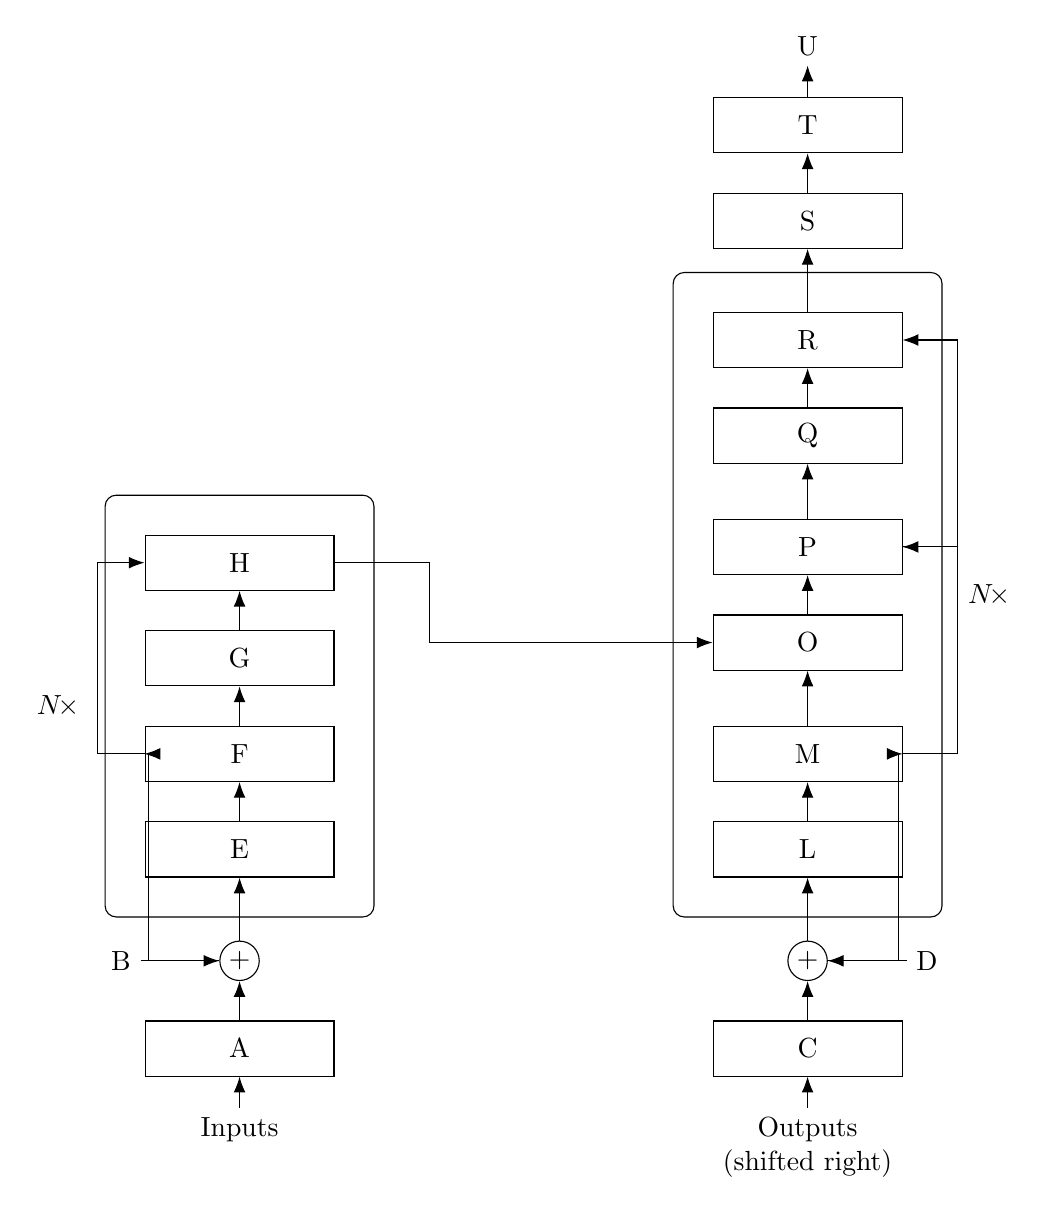
\begin{tikzpicture}[
  node distance=5mm,
  box/.style={draw,minimum width=24mm,minimum height=7mm,align=center},
  plus/.style={draw,circle,inner sep=0pt,minimum size=5mm},
  >={Latex[length=2mm]},
  every path/.style={draw,->,line width=.4pt}
]
% Encoder input
\node[box] (A) {A};
\node[plus,above=5mm of A] (pe) {$+$};
\node[left=10mm of pe] (B) {B};
\draw (B) -- (pe);
\draw (A) -- (pe);
\node[below=4mm of A] (in) {Inputs};
\draw (in) -- (A);

\node[box,above=8mm of pe] (E) {E};
\node[box,above=of E] (F) {F};
\node[box,above=of F] (G) {G};
\node[box,above=of G] (H) {H};
\draw (pe) -- (E); \draw (E) -- (F); \draw (F) -- (G); \draw (G) -- (H);
\draw (pe.west) -- ++(-9mm,0) |- (F.west);
\draw (F.west) -- ++(-6mm,0) |- (H.west);
\node[draw,rounded corners,fit=(E)(H),inner sep=5mm] (enc) {};
\node[left=2mm of enc] {$N\!\times$};

% Decoder input
\node[box,right=48mm of A] (C) {C};
\node[plus,above=5mm of C] (pd) {$+$};
\node[right=10mm of pd] (D) {D};
\draw (D) -- (pd); \draw (C) -- (pd);
\node[below=4mm of C,align=center] (out) {Outputs\\(shifted right)};
\draw (out) -- (C);

\node[box,above=8mm of pd] (L) {L};
\node[box,above=of L] (M) {M};
\node[box,above=7mm of M] (O) {O};
\node[box,above=of O] (P) {P};
\node[box,above=7mm of P] (Q) {Q};
\node[box,above=of Q] (R) {R};
\draw (pd) -- (L); \draw (L) -- (M); \draw (M) -- (O); \draw (O) -- (P); \draw (P) -- (Q); \draw (Q) -- (R);
\draw (pd.east) -- ++(9mm,0) |- (M.east);
\draw (M.east) -- ++(7mm,0) |- (P.east);
\draw (P.east) -- ++(7mm,0) |- (R.east);
\draw (H.east) -- ++(12mm,0) |- (O.west);
\node[draw,rounded corners,fit=(L)(R),inner sep=5mm] (dec) {};
\node[right=2mm of dec] {$N\!\times$};

\node[box,above=8mm of R] (S) {S};
\node[box,above=of S] (T) {T};
\node[above=4mm of T] (U) {U};
\draw (R) -- (S); \draw (S) -- (T); \draw (T) -- (U);
\end{tikzpicture}
\end{center}

\q{2}{Short Answer}
In the given Transformer architecture for one Encoder Decoder block, identify every Add \& Norm layer. Submit the corresponding component alphabets in alphabetical (ascending) order as a single uppercase string without spaces, commas, or quotation marks.

Example: If the correct components are Q, G, and S, your answer should be GQS.

\q{3}{MCQ}
Identify the function of component ``L'' in the given Transformer architecture.

\opts
\begin{enumerate}[label=(\alph*)]
\item Positional Encoding
\item Feed-Forward Network
\item Masked Multi-Head Self-Attention
\item Multi-Head Cross-Attention
\item Linear Output Projection
\end{enumerate}

\q{4}{MSQ}
Based on the architecture shown in the given image, identify all components that appear more than once. Assume the architecture contains exactly one Encoder block and one Decoder block.

\opts
\begin{enumerate}[label=(\alph*)]
\item Positional Encoding
\item Feed-Forward Network
\item Masked Multi-Head Self-Attention
\item Multi-Head Cross-Attention
\item tokenizer
\item Add \& Norm
\end{enumerate}

\q{5}{MSQ}
A researcher is exploring an alternate approach to implement masked attention in the transformer decoder. The causal mask considered is a binary lower-triangular matrix $M$ (where $M_{ij}=1$ for $j\le i$ and 0 otherwise). This mask ($M$) is applied as an element-wise multiplication ($\odot$) \textbf{after the softmax operation} on Attention Matrix ($A$):
\[
\operatorname{softmax}(A)\odot M.
\]
Identify the correct statements from the following:

\opts
\begin{enumerate}[label=(\alph*)]
\item The approach violates the autoregressive property.
\item The approach ensures autoregressive property is not violated by ensuring that the final attention weights of future tokens are 0.
\item The final attention weights in the new approach will be greater than or equal to that of the original approach.
\item The attention weights for the final token of the sequence will always be the same for both the approaches.
\end{enumerate}

\q{6}{MSQ}
Which of the following options correctly reflect the internal state updates performed during a Byte Pair Encoding (BPE) training iteration?

\opts
\begin{enumerate}[label=(\alph*)]
\item After a pair is chosen for merging, it is permanently added to the active vocabulary list.
\item The algorithm recalculates the log probability of the entire corpus before the next iteration.
\item The independent frequencies of the two constituent tokens that were part of the merge are reduced by the frequency of the merged token.
\item The original constituent tokens of the merged pair are removed from the vocabulary to optimize dictionary size.
\end{enumerate}

\q{7}{MSQ}
A baseline T5 model with denoising objective on a span of corrupted tokens is used for unsupervised pre-training. Consider the phrase ``life is like a box of chocolates''. If the word ``life'' and the span ``box of chocolates'' are selected for corruption, which of the following statements correctly describe the training process?

\opts
\begin{enumerate}[label=(\alph*)]
\item The input sequence replaces the corrupted spans with unique sentinal tokens as: ``<X> is like a <Y>''.
\item The output sequence generated takes the form ``<X> life <Y> box of chocolates <Z>'', with the final sentinal token to indicate sequence completion.
\item The loss is calculated exclusively over the generated sentinal tokens and the missing text.
\item The decoder reconstructs the entire original sequence autoregressively to compute the total loss over all positions.
\end{enumerate}

\q{8}{MCQ}
During the fine-tuning of GPT-1 for Textual Entailment tasks, what is the purpose of the delimiter token (\texttt{\$})?

\opts
\begin{enumerate}[label=(\alph*)]
\item To trigger the softmax function.
\item To separate premise and hypothesis.
\item To mark the end of the sentence.
\item To initialize the linear head.
\end{enumerate}

\q{9}{MCQ}
During the fine-tuning of a decoder-only Transformer for sequence classification, why is the hidden representation of the final input token used as the input to the classification layer?

\opts
\begin{enumerate}[label=(\alph*)]
\item The first token's representation relies exclusively on absolute positional encodings and lacks semantic context for classification.
\item The final token's representation is computed independently of self-attention, making its gradients more stable during the fine-tuning process.
\item Selecting the final token aligns with the autoregressive objective, eliminating the need for teacher forcing during the classification forward pass.
\item Causal self-attention ensures that only the final token's representation aggregates information from all preceding tokens in the sequence.
\end{enumerate}

\q{10}{MCQ}
In the decoding phase of a Language model, temperature scaling with $\tau=5$ is applied to the output logits before performing top-$p$ (nucleus) sampling. Which of the following options best describes the impact of the temperature scaling on the subsequent sampling step?

\opts
\begin{enumerate}[label=(\alph*)]
\item Increases the required number of candidate tokens thus expanding the nucleus.
\item Decreases the required number of candidate tokens thus shrinking the nucleus.
\item Truncates the tail of the distribution causing the sampling to behave similar to top-$k$ sampling.
\item Size of the nucleus remains unaffected by the temperature scaling as it only depends on order of the tokens.
\end{enumerate}

\q{11}{MCQ}
In the WordPiece tokenization algorithm, how does the scoring formula prioritize token merges?

\opts
\begin{enumerate}[label=(\alph*)]
\item It evaluates the log-probability of the pair and selects the highest scoring transition.
\item It merges the pair with the highest absolute frequency in the corpus.
\item It prioritizes pairs that occur together frequently but rarely appear independently in the corpus.
\item None of these.
\end{enumerate}

\q{12}{MCQ}
Consider the T5 ``text-to-text'' paradigm. How does the model process fundamentally different tasks such as Semantic Similarity (continuous regression) and Sentiment Analysis (discrete classification) during the fine-tuning phase?

\opts
\begin{enumerate}[label=(\alph*)]
\item The model uses the encoder to output the regression score and decoder for the classification tokens switching based on the input prompt.
\item The decoder part of the model is appended with separate prediction heads for regression and classification which are updated based on Mean Squared Error and Cross-Entropy respectively.
\item The model treats both tasks as sequence generation objectives with task-specific prefix added in the input and all output is generated as strings.
\item None of these.
\end{enumerate}

\q{13}{MCQ}
In the context of the BART (Bidirectional AutoRegressive Transformer) architecture, how does the model handle corrupted input sequences compared to its output?

\opts
\begin{enumerate}[label=(\alph*)]
\item The decoder ignores the encoder output and performs standard causal language modeling.
\item The encoder processes the original sequence and the decoder predicts the corrupted tokens.
\item The encoder processes the corrupted sequence and the decoder predicts the entire original sequence.
\item Both the encoder and decoder process the corrupted sequence to calculate masked loss.
\end{enumerate}

\q{14}{MCQ}
When comparing the C4 dataset to an ``Unfiltered-C4'' dataset that is 8 times larger, what was the observed effect on downstream task performance?

\opts
\begin{enumerate}[label=(\alph*)]
\item Performance remained identical, suggesting a saturation point in data utility.
\item Performance improved only for high-resource tasks like translation.
\item Performance improved significantly due to the increased diversity of data.
\item Performance degraded across all tasks despite the larger scale.
\end{enumerate}

\q{15}{MCQ}
Which of the following describes the ``Adapter Layers'' fine-tuning strategy?

\opts
\begin{enumerate}[label=(\alph*)]
\item Randomly freezing 50\% of the attention heads in each layer during training.
\item Adding small dense-ReLU-dense blocks after FFN layers and updating only those and Layer Norm parameters.
\item Updating all parameters in the model but using a much smaller learning rate.
\item Increasing the dimension $d_{model}$ of the existing Feed-Forward networks.
\end{enumerate}

\q{16}{MCQ}
Which of the following is a reported negative effect of including significantly duplicated content in LLM training data?

\opts
\begin{enumerate}[label=(\alph*)]
\item It decreases the model's overall inference speed during deployment.
\item It causes the model to generate repeated sequences much more frequently.
\item It permanently reduces the maximum supported context window length.
\item It causes the model to lose the ability to process multilingual input.
\end{enumerate}

\q{17}{MCQ}
If you have a fixed compute budget ($C$) and choose to train an extraordinarily large model (massive $N$) on a relatively small dataset (small $D$), what is the likely outcome according to scaling laws?

\opts
\begin{enumerate}[label=(\alph*)]
\item The model will be over-trained and memorize the dataset.
\item The model will be under-trained and less capable than a smaller model trained on more data with the same compute budget.
\item The model will perfectly memorize the small dataset and generalize flawlessly.
\item The model's inference speed will increase dramatically.
\end{enumerate}

\contexthead{18--19}
Consider the following corpus consisting of 4 words (ignore spaces and punctuation):
\[
\text{there is no spoon}
\]
The vocabulary is constructed using the whole words in this corpus and the individual characters in this corpus. The vocabulary should now have 13 tokens. Use this vocabulary for the given subquestions.

\q{18}{MSQ}
Using the vocabulary constructed, two new continuous strings: ``prison'' and ``rhino'' are to be segmented. Which of the following proposed segmentations are valid?

\opts
\begin{enumerate}[label=(\alph*)]
\item prison
\item p, r, is, o, n
\item p, r, is, on
\item r, h, i, n, o
\item r, h, i, no
\end{enumerate}

\q{19}{MCQ}
Using a unigram language model, identify the segment with the highest probability from the given options:

\opts
\begin{enumerate}[label=(\alph*)]
\item n, o, i, s, e, s
\item no, is, e, s
\item nois, e, s
\item no, i, s, e, s
\end{enumerate}

\end{document}
